\documentclass[11pt,letterpaper,oneside]{article}
\usepackage{fullpage}
\usepackage{setspace}
%\usepackage{subfiles}
\usepackage{hyperref}
\usepackage{parskip}
\usepackage{mdframed}
\usepackage{caption}
\usepackage{graphicx}

\newenvironment{aside}
  {\begin{mdframed}[style=0,%
      leftline=false,rightline=false,leftmargin=2em,rightmargin=2em,%
          innerleftmargin=0pt,innerrightmargin=0pt,linewidth=0.75pt,%
      skipabove=7pt,skipbelow=7pt]\small\vspace{0.1cm}}
  {\end{mdframed}}
  
\newenvironment{tabover}
  {\begin{mdframed}[style=0,%
      leftline=false,rightline=false,leftmargin=2em,topline=false,bottomline=false,rightmargin=2em,innertopmargin=0em,skipabove=0pt,%
          innerleftmargin=0pt,innerrightmargin=0pt]}
  {\end{mdframed}}


\newcommand{\file}[1]{{{\texttt{#1}}}}
\newcommand{\cmdline}[1]{{{\mbox{\texttt{#1}}}}} 
\newcommand{\classname}[1]{{{\texttt{#1}}}} 
  
\begin{document}

\title{User Guide for Auto-WEKA 0.5
}

\author{
Chris~Thornton \& Frank~Hutter\\
Department of Computer Science\\
University of British Columbia\\
Vancouver, BC\ \ V6T~1Z4, Canada\\
\texttt{\{cwthornt,hutter\}@cs.ubc.ca}
}

\maketitle

\tableofcontents

%%%%%%%%%%%%%%%%%%%%%%%%%%%%%%%%%%%%%%%%%%%
\section{Introduction}\label{sec:intro}
%%%%%%%%%%%%%%%%%%%%%%%%%%%%%%%%%%%%%%%%%%%



Auto-WEKA is a tool that performs combined algorithm selection and hyperparmeter optimisation over the classification and regression algorithms implements in WEKA. More specifically, given a specific dataset, Auto-WEKA explores hyperparameter settings for many algorithms and recommends to a user which method will likely have good generalization performance, using model based optimisation techniques.

%\begin{aside}
% This version of Auto-WEKA is research quality code, and there are still a few steps that are a bit cumbersome.  We are working at making this process much smoother, and any help in fixing these problems is greatly appreciated!
%\end{aside}

%%%%%%%%%%%%%%%%%%%%%%%%%%%%%%%%%%%%%%%%%%%%%%%%%%%%%%%%%%%%%%%%%%%%
\subsection{License}
%%%%%%%%%%%%%%%%%%%%%%%%%%%%%%%%%%%%%%%%%%%%%%%%%%%%%%%%%%%%%%%%%%%%

Auto-WEKA is open source software issued under the \href{http://www.gnu.org/licenses/gpl.html}{GNU General Public License}. Note that each of the optimisation methods that Auto-WEKA have their own license that govern their use.

\subsection{Prerequisites}

Auto-WEKA itself requires only Java 6 or newer to run, while the underlying optimisers that Auto-WEKA uses may have other requirements. Auto-WEKA was developed on Unix-compatible operating systems, but also runs on Windows. Auto-WEKA can use any version of \href{http://www.cs.waikato.ac.nz/ml/weka/}{WEKA}, but it has been targeted against 3.7.9. 

Auto-WEKA makes use of a few modifications to the algorithms in WEKA, detailed inside the \file{autoweka.patch} provided. You can apply the patch to your own WEKA distribution by running \cmdline{patch -Np1 < autoweka.patch} from the WEKA source directory. The changes in this patch just add a support for algorithms to detect if the thread that they have been running in has been interrupted, and then break out of their training phase at their earliest convenience. We have provided a pre-compiled version of WEKA with the patches applied for you to use if you do not wish to compile your own version.

\begin{aside}
Note that you can still use an unmodified version of WEKA, just that you will likely get inferior performance; if Auto-WEKA tries to run a method that takes more than your allotted time budget, it will be equivalent to a method that wasn't able to get a single correct result, while the modified method will report a result that may not be trained to optimality. 
\end{aside}


\subsection{Included Versions}

The Auto-WEKA distribution comes with a ``standalone'' and ``light'' version of Auto-WEKA. The standalone version (found in \file{autoweka.jar}) contains the patched version of WEKA, along with the dependencies that are needed for the GUI. The light version (found in \file{autoweka-light.jar}) \ contains just the Auto-WEKA classes, so you will have to add the WEKA classes (and optionally the classes for the GUI) manually on the class path. Sample scripts that demonstrate how to do this can be found in \file{scripts/autoweka} depending on your platform.

Auto-WEKA makes use of a number of configuration files provided in the \file{params} directory, so you should ensure that you should keep this directory in the same place as either \file{autoweka.jar} or \file{autoweka-light.jar}.


%%%%%%%%%%%%%%%%%%%%%%%%%%%%%%%%%%%%%%%%%%%
\section{Auto-WEKA Overview}\label{sec:overview}
%%%%%%%%%%%%%%%%%%%%%%%%%%%%%%%%%%%%%%%%%%%

Using Auto-WEKA can be broken down into three main steps. First, you have to build your experiment definition, which tells Auto-WEKA what dataset(s) to run on, as well as what kind of hyperparameter search will be done (either through a model based method, or through something like grid search). Once the definition has been written, the experiment needs to be fully instantiated by having Auto-WEKA detect what kind of classifiers can be used given the definition you wrote. At this stage, Auto-WEKA also resolves all path names to absolute paths, so instantiated experiments may have some difficulty when being moved between different computation environments.  

Once an experiment has been produced, it actually has to be executed. Auto-WEKA takes advantage of multiple cores by running the same experiment with different random seeds, the only requirement is that all the experiments have a similar file system (since Auto-WEKA relies on absolute path names). The user has to start a new run of the experiment for each seed/core that they want to take advantage of.

After the experiment has been executed, the analysis phase occurs. When Auto-WEKA uses a model based optimisation method, it produces a trajectory of hyperparameters that were identified by the optimisation method as being the best at a particular point in time. The simplest form of analysis looks at the best hyperparameters that were found across all seeds, and uses the trained model to make predictions on a new dataset. Additional experiments can be performed on these trajectory points, for example to see if all the trajectory points have a similar performance on a new set of data that the optimisation method did not have access to.

The above three steps can all be completed through the use of a GUI (see Section~\ref{sec:gui}), or through the more flexible command line interface (see Sections~\ref{sec:defining}-\ref{sec:analyzing}).

%%%%%%%%%%%%%%%%%%%%%%%%%%%%%%%%%%%%%%%%%%% 
\section{Using the GUI}\label{sec:gui}
%%%%%%%%%%%%%%%%%%%%%%%%%%%%%%%%%%%%%%%%%%%

Auto-WEKA contains a GUI to allow for easy execution of experiments. To launch the GUI, you need to execute the class \classname{autoweka.ui.Launcher}. This can be done by running the command \cmdline{java -jar autoweka.jar}, or using one of the Auto-WEKA scripts. This brings up the following window that allows you to configure your experiment, run your experiment, and finally get the best set of hyperparameters that were found. Auto-WEKA features a wizard mode that uses presets to help get experiments running as quick as possible. Additionally, the launcher also provides a shortcut to launching the standard WEKA UI.

\begin{center}
  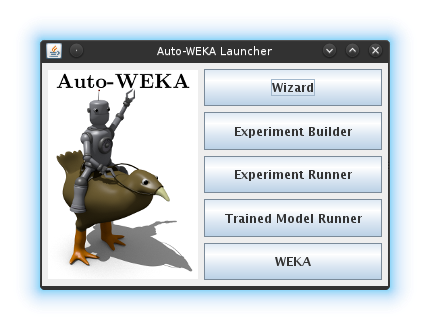
\includegraphics[scale=0.75]{guiscreens/launcher.png}
\end{center}


\subsection{Wizard}

The wizard allows for easy execution of experiments, targeted towards use cases where minimal input is required from the user. After pointing the wizard at the training data (in WEKA's ARFF data format), the user just has to pick the preset that best suits their resource limits. (Note that for larger datasets,  you will not achieve good results by using very small time limits). Pressing the ``Run Experiment'' button will cause Auto-WEKA to use the optimisation method SMAC (See Section~\ref{sec:smbo}) to find hyperparemter settings with good accuracy (for classification) or RMSE (for regression). Once the optimisation has completed, the wizard will indicate what method and hyperparameters were selected, and allow for predictions on new datasets using the trained method.

\begin{center}
  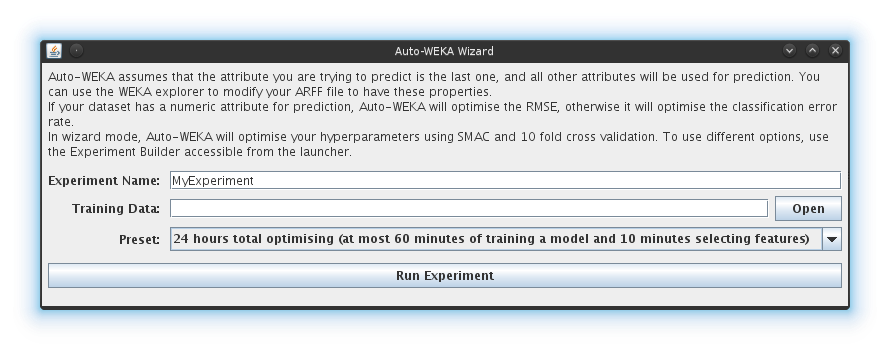
\includegraphics[scale=0.7]{guiscreens/wizard.png}
\end{center}

\subsection{Experiment Builder}

The Experiment Builder has three pages. On the first page, you specify the the location of the training data in the ARFF format. Auto-WEKA GUI assumes that the attribute you are attempting to predict is last attribute in the file,  you may need to use the WEKA UI to reorder your dataset. Additionally, you can specify the test data to use (this is only ever used in the analysis stage). If you do not specify any test data, Auto-WEKA just uses the training data instead. You can also set up the way that the optimisation method will use the training data,  through the use of an ``instance generator''. After picking the desired method, you can fine tune the method's settings by clicking on the ``Edit'' button. A more detailed explanation of each instance generator and its associated options can be found in Section~\ref{sec:instancegenerators}. Once you have made your choices, press the ``Next'' button.

\begin{center}
  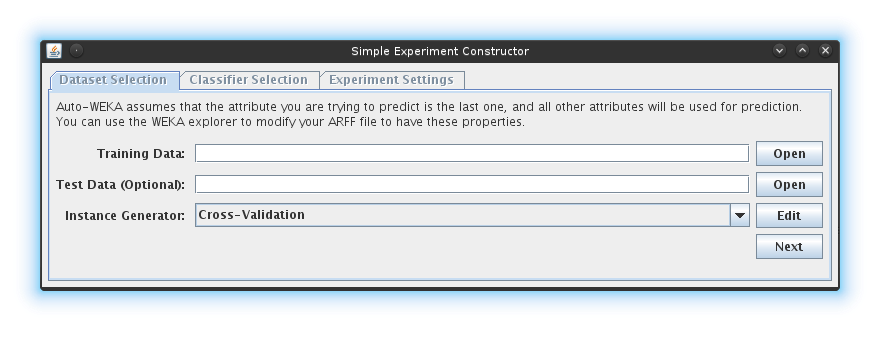
\includegraphics[scale=0.7]{guiscreens/builder-dataset.png}
\end{center}

Next Auto-WEKA allows you to limit the choice of classifiers that it will consider during for the SMBO method. The second page allows you to select which methods you would like, by control/shift clicking on the different class names to limit your selection. We recommend that you should keep all the methods selected unless you have a very specific reason for not using a particular method. Detailed about which classifiers are not applicable are printed to the system console. Once you have made your selections,  press the ``Next'' button.

\begin{center}
  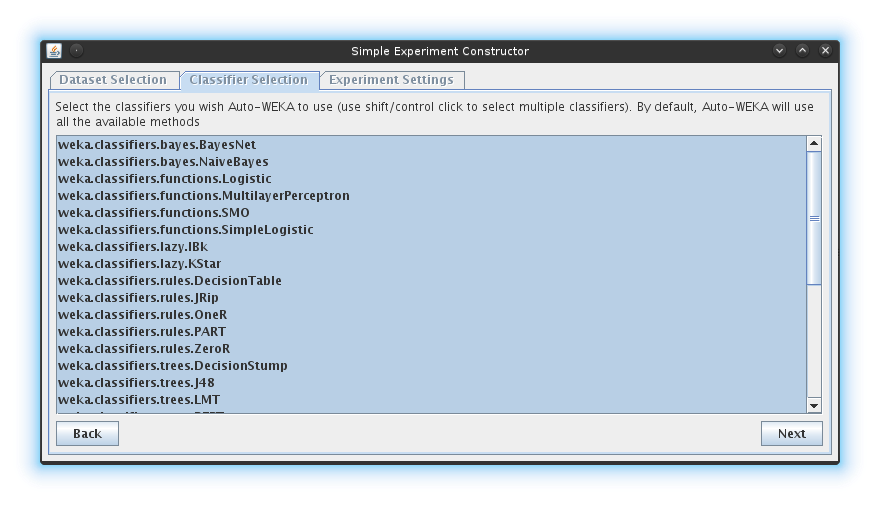
\includegraphics[scale=0.7]{guiscreens/builder-classifier.png}
\end{center}

The last page allows you to specify your experiment settings. The ``output folder'' is the folder where the sub-folder containing all of the experiment data will be produced. Change the ``Result Metric'' to one that is applicable to your dataset. After you select your optimisation method, you can fine tune specific settings by clicking on the edit button. These settings are detailed for each  method in Section~\ref{sec:smbo}. The Optimisation timeout is the number of hours that you are willing to give the optimiser to perform the hyperparameter search. The training memory limit and training run timeout are the resource constraints that are placed on the individual run of a classification or regression method that the optimisation method will perform (and it should be allowed to perform many of them). The attribute selection check box indicates to Auto-WEKA if the hyperparameter search should also be performed over WEKA's methods for transforming/selecting attributes in the dataset. The attribute selection timeout is only used when attribute selection is enabled, and is the maximum number of minutes that will be used to perform the attribute selection for each run of a hyperparameter configuration.

\begin{center}
  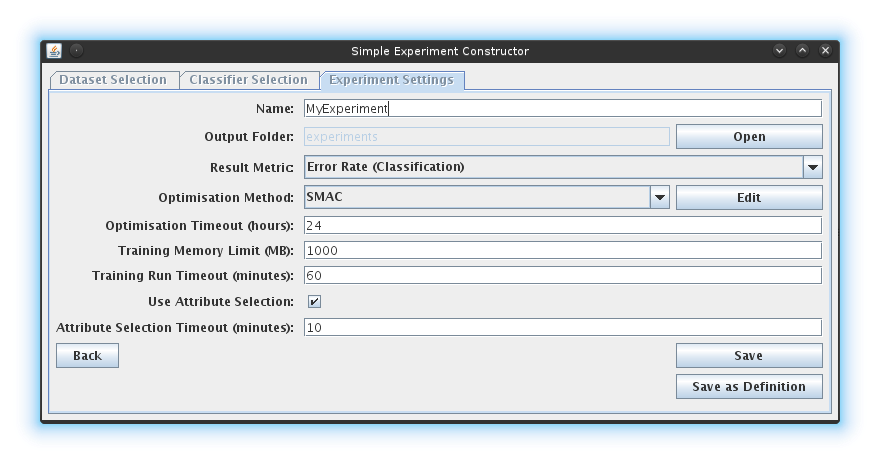
\includegraphics[scale=0.7]{guiscreens/builder-experiment.png}
\end{center}

Finally, you can either choose to fully instantiate the experiment by clicking on the ``Save'' button (which converts all paths to absolute paths) and sets up the folders for the experiment,  or you can choose to create a portable experiment definition by clicking the ``Save as Definition'' button. The experiment definition file can then be moved to a different environment,  or be modified to facilitate batch experiments. See Section~\ref{sec:experimentdefs} for more details.

\subsection{Experiment Runner}

The experiment runner provides an easy way to run a fully instantiated Auto-WEKA experiment. Simply select the folder containing the \file{.experiment} file, enter in a integer for a seed, and push the run button. For example, if your directory structure looks as follows:
\begin{verbatim}
  experiments/
     MyExperiment/
        MyExperiment.experiment
        ....
\end{verbatim}
The folder \file{experiments/MyExperiment} should be selected in the open file dialog.

\begin{center}
  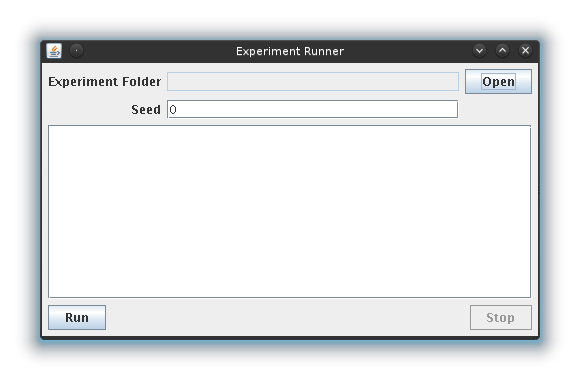
\includegraphics[scale=0.7]{guiscreens/runner.png}
\end{center}

After pressing the run button, the log screen will begin filling up with the output of the optimisation method. Consult the documentation that came with the optimisation method for an explanation of what appears.

Once the time budget has been exhausted, Auto-WEKA will begin training a model using all the training data and the best hyperparameters. If a testing set was provided, Auto-WEKA will print out some basic statistics on the performance of the trained model on the data.

\begin{aside}
  Sometimes the Stop button doesn't succeed in terminating the running process - if this is the case, you'll have to use the various tools of your OS to ensure that the optimisation process is terminated.
\end{aside}

\subsection{Trained Model Runner}

Since Auto-WEKA exploits parallelism by running the optimisation method with different seeds, after running your experiment a few times with unique seeds, you'll want to use the best hyperparameters found to make predictions on new data. After opening up the folder containing the \file{.experiment}, Auto-WEKA selects the hyperparameters that have the best error estimate. The hyperparameters are then displayed, so you can use them in WEKA's explorer (if you right click on any of the text boxes that contain arguments,  WEKA allows you to insert the command line string into it).

\begin{center}
  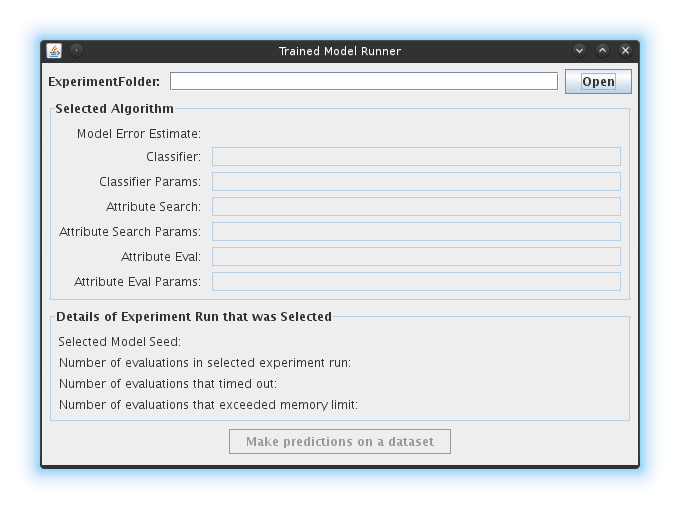
\includegraphics[scale=0.65]{guiscreens/modelrunner.png}
\end{center}

Additionally, you can provide new datasets (in ARFF format),  and use the trained model to make predictions (the results are saved as a CSV). If attribute selection was used,  this will be applied to the dataset before it is passed off to the model. Note that the format of the testing set needs to match the format of the training data exactly, otherwise you will likely get very strange predictions/cryptic error messages. 

%%%%%%%%%%%%%%%%%%%%%%%%%%%%%%%%%%%%%%%%%%% 
\section{Defining Experiments}\label{sec:defining}
%%%%%%%%%%%%%%%%%%%%%%%%%%%%%%%%%%%%%%%%%%%
 
If not using the GUI, Auto-WEKA can define experiments either on the command line through a rather tedious process (only documented in the code), or `experiment definition batches' can be made. An experiment definition batch is an XML file that contains a list of datasets to perform experiments on, and one or more experiment prototypes that contain information such as the type of optimisation method to use or the way to partition the provided training data. These files were designed for performing large comparisons of different settings on multiple datasets, but they can easily be applied to situations where you have a single dataset. Section~\ref{sec:experimentdefs} provides a description of how to write these files, but you can also look at the \classname{autoweka.ExperimentBatch} class and its JavaDocs to see how to use them. The GUI also provides a way to generate a simple version of these files, which you can then modify by hand. These experiment definitions also select the choice of optimisation method (see section~\ref{sec:smbo}), and the way to partition the training data using an `InstanceGenerator' (see section~\ref{sec:instancegenerators}).

Once the experiment definition has been created, Auto-WEKA needs to know what type of classification or regression algorithms and feature/attribute selection methods to used. These are all specified in \file{.param} files, detailed in section~\ref{sec:paramfiles}.

After the experiment definition is fully written, the main method of \classname{autoweka.ExperimentConstructor} can be invoked on the experiment definition file to determine which algorithms can be used on your datasets, and will generate the files needed under the \file{experiments} folder from the current working directory. 

\begin{aside}
  Using the provided script, this command can be executed as follows: \\
  \cmdline{scripts/autoweka autoweka.ExperimentConstructor path/to/experimentbatch.xml}
\end{aside}


%%%%%%%%%%%%%%%%%%%%%%%%%%%%%%%%
\subsection{Experiment Definition Files}\label{sec:experimentdefs}
%%%%%%%%%%%%%%%%%%%%%%%%%%%%%%%%

Experiment definitions are done in XML files, with a root node of an \texttt{experimentBatch}. Inside the experiment batch, there can be any number of \texttt{datasetComponent} and \texttt{experimentComponent} elements - this allows for quickly making experiments with multiple different settings on a variety of datasets. You can produce a template file by running the main method \texttt{autoweka.ExperimentBatch} with the name of the template file you wish to create, or saving a definition from the GUI.

\subsubsection{datasetComponent}

The \texttt{datasetComponent} defines a dataset that you want to perform experiments on. Auto-WEKA can take two formats for input. The first requires that datasets are a compressed zip containing exactly two files, \texttt{train.arff} and \texttt{test.arff}. Auto-WEKA will perform all of its experiments on the training data in \texttt{train.arff}, and will use the test data in \texttt{test.arff} for analysis after the experiment has completed. (If you don't have any test data, you can just create a dummy dataset file or use the training data again). A \texttt{datasetComponent} has the following form in the XML file with self explanatory names

\begin{verbatim}
<datasetComponent>
  <zipFile>path/to/zip/file.zip</zipFile>
  <name>DatasetName</name>
</datasetComponent>
\end{verbatim}

Additionally, Auto-WEKA can be pointed to the \texttt{train.arff} and \texttt{test.arff} individually. These datasetCompoments have the following form

\begin{verbatim}
<datasetComponent>
  <trainArff>path/to/train.arff</trainArff>
  <testArff>path/to/train.arff</testArff>
  <name>DatasetName</name>
</datasetComponent>
\end{verbatim}

\subsubsection{experimentComponent}\label{sec:experimentdefs:excomp}

The \texttt{experimentComponent} element contains the parameters that you want to use in an experiment on all of the \texttt{datasetComponent}s defined in the same file. 

\begin{verbatim}
<experimentComponent>
  <name>SMAC-CV10</name>
  <resultMetric>errorRate</resultMetric>
  <experimentConstructor>autoweka.smac.SMACExperimentConstructor</experimentConstructor>
  <instanceGenerator>autoweka.instancegenerators.CrossValidation</instanceGenerator>
  <instanceGeneratorArgs>numFolds=10:seed=0</instanceGeneratorArgs>
  <tunerTimeout>108000</tunerTimeout>
  <trainTimeout>9000.0</trainTimeout>
  <attributeSelection>true</attributeSelection>
  <attributeSelectionTimeout>900</attributeSelectionTimeout>
  <memory>3072m</memory>
  <extraProps></extraProps>
</experimentComponent>
\end{verbatim}
    
    
\begin{description}
 \item [name] The name of the experiment component, this will be combined with the data set when the full experiment is created.
 \item [resultMetric] The resultMetric to use. Most likely \texttt{errorRate} for classification. \texttt{rmse}, \texttt{rrse}, \texttt{meanAbsoluteErrorMetric} and  \texttt{relativeAbsoluteErrorMetric} are also supported. See the source for \classname{autoweka.ClassifierResult} for more.
 \item [experimentConstructor] The name of the class to be used to build the experiment - see \ref{sec:smbo} for a list of what values are supported.
 \item [instanceGenerator] The name of the class to be used for partitioning the training data, see \ref{sec:instancegenerators} for what classes are implemented.
 \item [instanceGeneratorArgs] A property string (\texttt{var1=val1:var2=val2...}) with arguments to the instance generator.
 \item [tunerTimeout] The number of seconds to run the optimisation method.
 \item [trainTimeout] The number of seconds to spend training an algorithm with a set of hyperparameters on a given partition of the training set.
 \item [attributeSelection] \texttt{true} if you want to consider using different feature/attribute selectors, \texttt{false} otherwise (or don't include it).
 \item [attributeSelectionTimeout] Number of seconds to spend doing feature/attribute selection.
 \item [memory] The memory limit that is passed to the Java instance that is training the classifier or regression method
 \item [extraProps] Optional extra arguments that can be passed to an experiment
 \item [allowedClassifiers] Optional argument that restricts what methods can be considered. Specify it multiple times to include a subset of methods, or don't specify it at all to make Auto-WEKA chose all possible methods.  
\end{description}

It is also possible to indicate in an experiment if some extra computations should be done on all points in the trajectory during the analysis stage. In your \texttt{experimentComponent}, you can create any number of \texttt{trajectoryPointExtras}:

\begin{verbatim}
<trajectoryPointExtras>
  <name>humanReadableName</name>
  <instance>instanceString</instance>
</trajectoryPointExtras>
\end{verbatim}

Here, the \texttt{name} is a human readable name the corresponds to the \texttt{instanceString} that is being executed. The instance string is what is passed to the instance generator, covered in section~\ref{sec:instancegenerators}. For example, if you want to see how the selected hyperparameters perform over time, you can add the following into your \texttt{experimentComponent}.% The contents of the \texttt{instance} node are explained in Section~\ref{sec:instancegenerators}.

\begin{verbatim}
<trajectoryPointExtras>
  <name>Test Performance</name>
  <instance>default</instance>
</trajectoryPointExtras>
\end{verbatim}

%%%%%%%%%%%%%%%%%%%%%%%%%%%%%%%%
\subsection{Instance Generators}\label{sec:instancegenerators}
%%%%%%%%%%%%%%%%%%%%%%%%%%%%%%%%

Auto-WEKA uses an instance generator to partition the training and test data provided into new sets of training and test data for the optimisation method to use, e.g. the training data is broken up into 10 folds in cross validation. Each partition of the data is called an `instance', and can be specified through a string, often in the form of a property string (\texttt{var1=val1:var2=val2:...}). Additionally, each Instance Generator also has a string of \texttt{instanceGeneratorArgs} that determine what instances will be created in your experiment. For the most common instance generators Auto-WEKA provides, these strings are detailed below.

\begin{aside}
The instance string \texttt{default} however has a the special meaning that the training and test data are unmodified.
\end{aside}

\subsubsection{Default}

The most boring of instance generators - it does nothing to the input training and test data, it ignores any arguments and returns the unmodified partition of instances.

\subsubsection{Cross Validation}

Performs $k$-fold cross validation on the training set. Implemented in \\ \texttt{autoweka.instancegenerators.CrossValidation}. 

\textbf{Generator Args}:
\begin{tabover}
A property string containing the following two elements:
\begin{description}
 \item [seed] The seed to use for randomizing the dataset
 \item [numFolds] The number of folds to generate
\end{description}
\end{tabover}

\textbf{Instance String}
\begin{tabover}
A property string containing the following three elements:
\begin{description}
 \item [seed] The seed to use for randomizing the dataset
 \item [numFolds] The number of folds total
 \item [fold] The instance's fold number
\end{description}
\end{tabover}


\subsubsection{Random Sub-Sampling}

Performs generates an arbitrary number of folds by randomly making a partition of the training data of a fixed percentage. Implemented in \texttt{autoweka.instancegenerators.RandomSubSampling}. 

\textbf{Generator Args}:
\begin{tabover}
A property string containing the following the following elements:
\begin{description}
 \item [startingSeed] The seed to use for randomizing the dataset
 \item [numSamples] The number of subsamples to generate
 \item [percent] The percent of the training data to use as `new training data'
 \item [bias] Optional: The bias towards a uniform class distribution
\end{description}
\end{tabover}


\textbf{Instance String}
\begin{tabover}
A property string containing the following three elements:
\begin{description}
 \item [seed] The seed to use for randomizing the dataset
 \item [percent] The percent of the training data to use as `new training data'
 \item [bias] Optional: The bias towards a uniform class distribution
\end{description}
\end{tabover}

\subsubsection{Termination Holdout}

A meta instance generator that removes a random percentage of the training data before passing it on to the target instance generator. Implemented in \texttt{autoweka.instancegenerators.TerminationHoldout}. 

\textbf{Generator Args}:
\begin{tabover}
A string with three components, separated by \texttt{[\$]}. The first component contains the parameters for the holdout method (described below), while the second component contains the name of the target instance generator that will receive the subsampled dataset. The final component contains all the arguments that will be passed on to the generator of the target 
A property string containing the following the following elements:
\begin{description}
 \item [terminationSeed] The seed to use for randomizing the dataset
 \item [terminationPercent] The percent of the training data to use hold back
 \item [terminationBias] Optional: The bias towards a uniform class distribution
\end{description}
\end{tabover}

\textbf{Instance String}
\begin{tabover}
A string with three components, separated by \texttt{[\$]}. The first component contains the parameters for the holdout method (described below), while the second component contains the name of the target instance generator that will receive the subsampled dataset. The final component contains all the arguments that will be passed on to the generator of the target 
\begin{description}
 \item [terminationSeed] The seed to use for randomizing the dataset
 \item [terminationPercent] The percent of the training data to use as `new training data'
 \item [terminationBias] Optional: The bias towards a uniform class distribution
\end{description}
\end{tabover}

%%%%%%%%%%%%%%%%%%%%%%%%%%%%%%%%
\subsection{Optimisation Methods}\label{sec:smbo}
%%%%%%%%%%%%%%%%%%%%%%%%%%%%%%%%

Currently Auto-WEKA supports three different optimisation methods, the Tree based Parzen Estimator (TPE), Sequential Model-based Algorithm Configuration (SMAC) and Iterated F-Race (IRace). Each method requires some initial set up with Auto-WEKA so that it can be used smoothly, namely by creating \texttt{.properties} files that tell Auto-WEKA where to find each method (These files must be in the current working directory when you invoke any of the experiment constructor commands. The syntax of a properties file is of the form \texttt{var=value}, with one variable per line). Each of the following sections mentions how to tell Auto-WEKA to use SMBO method, as well as the name and contents of the \texttt{.properties} file that must be created.

\subsubsection{SMAC}

\href{http://www.cs.ubc.ca/labs/beta/Projects/SMAC/}{SMAC} was designed for algorithm configuration, but can easily be used in other cases of black box optimisation. The Auto-WEKA distribution comes with a development version of SMAC v2.06.01. To build an experiment with SMAC, you use the \texttt{autoweka.smac.SMACExperimentConstructor}. 

\textbf{autoweka.smac.SMACExperimentConstructor.properties}
\begin{description}
 \item[\texttt{smacexecutable}]: The path to the \file{smac} script (with no \texttt{.bat} extension on Windows) inside the SMAC distribution. 
\end{description}

\begin{aside}
A few of SMAC's options are also supported by Auto-WEKA (e.g. \texttt{initialIncumbent} and \texttt{executionMode}), look inside the \\\classname{autoweka.smac.SMACExperimentConstructor} class to see what variables are supported in the \texttt{extraProps} of an experiment definition.
\end{aside}

\subsubsection{TPE}

TPE is provided by the \href{http://jaberg.github.com/hyperopt/}{Hyperopt} project, written for Python 2.7. To build an experiment with TPE, you use the \texttt{autoweka.tpe.TPEExperimentConstructor}. 

\textbf{autoweka.smac.SMACExperimentConstructor.properties}
\begin{description}
 \item[\texttt{tperunner}]: Path to the \texttt{tperunner.py} file in the Auto-WEKA source directory
 \item[\texttt{python}] (Optional): The Python you want to use - defaults to trying to find a \texttt{python} on the system path.
 \item[\texttt{pythonpath}] (Optional): Sets the PYTHONPATH environment variable before invoking python (useful if you don't have hyperopt inside your site-packages).
\end{description}

\subsubsection{IRace}

\href{http://iridia.ulb.ac.be/irace/}{IRace} is another tool that was designed for algorithm configuration, with an implementation in R. To build an experiment with IRace, you use the \texttt{autoweka.irace.IRaceExperimentConstructor}. 
\begin{aside}
  Note that IRace defines its budget in terms of the number of evaluations of different hyperparmeter settings, not in total time. As such, the number of seconds that Auto-WEKA uses for the \texttt{tunerTimeout} will be used as the number of evaluations.
\end{aside}

\textbf{autoweka.smac.IRaceExperimentConstructor.properties}
\begin{description}
  \item[\texttt{iraceexecutable}]: Path to the \texttt{irace} script inside the R package.
\end{description}

%%%%%%%%%%%%%%%%%%%%%%%%%%%%%%%%
\subsection{Parameter Files}\label{sec:paramfiles}
%%%%%%%%%%%%%%%%%%%%%%%%%%%%%%%%

Auto-WEKA groups classification and regression algorithms into 3 categories: base, meta and ensemble. Meta methods are methods that take a single base method and use it to perform classification (like AdaBoost), while ensemble methods use a number of base methods to perform classification. Additionally, Auto-WEKA supports feature/attribute selection, through the use of search and evaluator methods. Many of these methods have parameters that influence their behaviour, and these parameters are exposed through the use of \texttt{.param} files. The name of the file contains the full class name of the method that we are exposing to Auto-WEKA (so for WEKA's SVM implementation, the file would be called \texttt{weka.classifiers.functions.SMO.params}), and it is placed inside the subfolder of the \texttt{params} directory corresponding to the method (so the SVM implementation goes inside the \texttt{base} subfolder, while the param file for AdaBoost would go inside the \texttt{meta} subfolder).

The contents of these files can be broken down into two parts: parameter definitions and conditional statements. For examples for a number of different classification, regression and feature selection methods, see the the provided \texttt{.param} files that come with Auto-WEKA.

\subsubsection{Parameter Definitions}

For each parameter exposed to Auto-WEKA is written on its own line, and has the following form. 
\begin{center}
 \texttt{<FLAGS>\_<NAME> <DOMAIN> <DEFAULT><TYPEFLAGS>}
\end{center}

\begin{description}
  \item[\texttt{FLAGS}] These will all be stripped by Auto-WEKA before they are passed to WEKA. The flags are defined up until the last underscore before the \texttt{NAME}. Summary of valid flags:
  \begin{description}
    \item[\texttt{HIDDEN}] The parameter will be never be seen by the WEKA method.
    \item[\texttt{INT}] The parameter will be forced to an integer when it is passed on to WEKA.
    \item[\texttt{QUOTE\_START}] A quote character will be inserted after this parameter, up until the next \texttt{QUOTE\_END}
    \item[\texttt{QUOTE\_END}] Inserts a quotation character and removes the parameter
    \item[\texttt{DASHDASH}] Inserts a double dash (\texttt{--}) into the call string
  \end{description}
  \item{\texttt{NAME}} The name of the argument that WEKA expects on the command line. Note that in most cases, these are single capital letters (and never contain an underscore)
  \item{\texttt{DOMAIN}} The domain of this parameter, which is either numeric or categorical.
  \begin{description}
    \item[Categorical] The domain is specified as a comma separated list of strings in between two curly braces, eg. \texttt{\{v1, v2, ... vk\}}
    \item[Numeric] The domain is specified as two comma separated numbers for the lower and upper range of the domain between two square brackets, eg. \texttt{[0.1, 10]}
  \end{description}
  \item[\texttt{DEFAULT}] The default value of the parameter (which must be inside the domain) is specified between two square brackets eg. \texttt{[1.0]}
  \item[\texttt{TYPEFLAGS}] Optional type flags for numeric domains. If you want to recommend to the SMBO method that this parameter should be treated as an integer, add an \texttt{i}. If the parameter should be sampled on a logarithmic scale, add a \texttt{l}
\end{description}

%EXAMPLE
For example, the parameter file for random forests contains the line:
\begin{verbatim}
  INT_I [2, 256][10]il
\end{verbatim}
This indicates that there is a parameter \texttt{I} that must be treated as an integer, with values ranging between 2 and 256 (a default value of 10), and should be sampled log-uniformly.

Additionally, Auto-WEKA defines special treatment to the categorical domain of \texttt{\{REMOVED, REMOVE\_PREV\}}, which can be best demonstarted through an example. Suppose we have a parameter \texttt{M} which is a flag of a classifier that enables aggressive memory caching. If \texttt{M} is set to \texttt{REMOVED}, by Auto-WEKA, then WEKA will receive the argument \texttt{-M}. In the case that \texttt{M} is set to \texttt{REMOVE\_PREV}, then Auto-WEKA will completely hide the \texttt{-M} flag from the WEKA classifier.

\begin{aside}
 Note: Arguments are sorted alphabetically by Auto-WEKA before they are passed on to the WEKA method.
\end{aside}

\subsubsection{Conditionals}

For many methods, only some parameters make sense once another parameter takes on a certain value. If this is the case, after all the parameters have been defined in the \texttt{.param} file, you need to inform Auto-WEKA of these conditionals. All conditionals must appear after a \texttt{Conditionals:} line. The format of a conditional line is as follows

\begin{center}
 \texttt{<PARAMETER> | <PARENT> in \{<VALUE1>, <VALUE2>, ...\}}
\end{center}

\begin{description}
  \item[\texttt{PARAMETER}] The name of the child parameter that is active based on the value of the parent
  \item[\texttt{PARENT}] The name of the parent parameter that the conditional depends on
  \item[\texttt{VALUE*}] If the parent parameter takes on one of the values in this list, then the child parameter will be enabled, Otherwise, the child parameter is disabled.
\end{description}


%\subsection{List Experiments}

%Auto-WEKA also supports additional types of experiments where all the hyperparameter/classifier combinations are fixed in advance, these experiments are implemented as \texttt{ListExperiments}. They have a nearly identical process for creation/execution as regular experiments, 
 
%%%%%%%%%%%%%%%%%%%%%%%%%%%%%%%%%%%%%%%%%%% 
\section{Running Experiments Using the CLI}\label{sec:running}
%%%%%%%%%%%%%%%%%%%%%%%%%%%%%%%%%%%%%%%%%%%

After generating your experiment using the main method of the \texttt{ExperimentConstructor}, execute the main method of \texttt{autoweka.Experiment} with two parameters - the path to the experiment folder and an initial seed for the random number generator of the SMBO method. Auto-WEKA has been designed to execute many optimisation runs in parallel, simply change the seed that you pass to each invocation of \texttt{autoweka.Experiment}. Auto-WEKA will now grind away for a while until the \texttt{tunerTimeout} has been hit as specified in the experiment definition.

Optionally, you can instead invoke the \classname{autoweka.tools.ExperimentRunner} with the same arguments as above. This class does the extra step at the end of an experiment to produce a trained model on the entire training dataset so that it can be easily used to make further predictions. (This class performs the same operations as the Experiment Runner window in the GUI).

\begin{aside}
 Once your generate the experiment by running the \classname{ExperimentConstructor}, Auto-WEKA tries to resolve path names fully, so it is unlikely that you can move these folders around and still run the experiment.
\end{aside}

 
%%%%%%%%%%%%%%%%%%%%%%%%%%%%%%%%%%%%%%%%%%% 
\section{Analyzing Experiments Using the CLI}\label{sec:analyzing}
%%%%%%%%%%%%%%%%%%%%%%%%%%%%%%%%%%%%%%%%%%%
The first step in doing any analysis of experiments is to generate the trajectories of the optimisation run. This can be done by invoking the \classname{autoweka.TrajectoryParser} class, with the arguments of the experiment folder and the seed you want to parse. This step is only required if you did not use the \classname{autoweka.tools.ExperimentRunner} to execute your experiment.

For each seed that the experiment was run with, there should be a file with the naming scheme of \texttt{<ExperimentName>.trajectories.<Seed>}. If you defined any \texttt{trajectoryPointExtras} in your experiment definition, you'll want to run the main method of \texttt{autoweka.TrajectoryPointExtraRunner} with the arguments \\\texttt{<ExperimentFolder>/<ExperimentName>.trajectories.<Seed>} before performing any other analysis. This does runs of the classifer/hyperparameters identified in the trajectory on whatever instance strings you've specified, and stores the result of the error metric and timing information into the trajectory file.

Once all the individual trajectory files are complete, each of these files needs to be merged into a single trajectory group for analysis. Run the main method of \texttt{autoweka.TrajectoryMerger}, with a single argument of the experiment's directory. This produces a single file \texttt{<ExperimentName>.trajectories} inside the experiment's folder.

Finally, to get the best hyper-parameters and method that Auto-WEKA has found on the dataset, run the main method of \texttt{autoweka.tools.GetBestFromTrajectoryGroup}, with the single command line argument pointing at the \texttt{.trajectories} file that was produced in the last step. This will print out information on how many trajectories were used to select the best, what Auto-WEKA thinks the performance of the selected method on the training set is, as well as which algorithm was chosen and the command line arguments that should be given to the algorithm.

%%%%%%%%%%%%%%%%%%%%%%%%%%%%%%%%%%%%%%%%%%% 
\section{CLI Sample Experiment Walkthrough}\label{sec:analyzing}
%%%%%%%%%%%%%%%%%%%%%%%%%%%%%%%%%%%%%%%%%%%
 
Include in the distribution is a sample experiment definition that runs SMAC on the German Credit dataset from the UCI repository, this section will show you how to run a typical Auto-WEKA experiment.

First, navigate to the \texttt{autoweka} directory that contains the \texttt{autoweka.jar} file. First, we need to build the actual experiment by running the \texttt{ExperimentConstructor}

\begin{aside}
 For all the following Java commands, we assume that you run them inside the \texttt{autoweka} directory, and add both \texttt{autoweka.jar} and \texttt{weka.jar} to the Java's class path.
\end{aside}

\begin{verbatim}
  java -cp autoweka.jar  autoweka.ExperimentConstructor sampleexperiment.xml
\end{verbatim}

This will load the dataset in \texttt{sampledata/creditg.zip}, determine what classifiers and feature selectors that are defined in the \texttt{params} directory can be used, and write out the experiment into the \texttt{experiments} directory.

\begin{aside}
 Note that you will have to modify \texttt{autoweka.smac.SMACExperimentConstructor.properties} to point to your distribution of SMAC, if you are not using the version that came bundled with Auto-WEKA.
\end{aside}

Next, we need to run our experiments by invoking the \texttt{Experiment} with different seeds

\begin{verbatim}
  java -cp autoweka.jar autoweka.Experiment experiments/SMAC-CV10-GermanCredit 0
  java -cp autoweka.jar autoweka.Experiment experiments/SMAC-CV10-GermanCredit 1
  java -cp autoweka.jar autoweka.Experiment experiments/SMAC-CV10-GermanCredit 2
  ...
\end{verbatim}

After watching some paint dry (and the experiments have completed), we now need to generate and combine all the trajectories into a single file using the \texttt{TrajectoryMerger}

\begin{verbatim}
  java -cp autoweka.jar autoweka.TrajectoryParser experiments/SMAC-CV10-GermanCredit 0
  java -cp autoweka.jar autoweka.TrajectoryParser experiments/SMAC-CV10-GermanCredit 1
  java -cp autoweka.jar autoweka.TrajectoryParser experiments/SMAC-CV10-GermanCredit 2
  ...
  java -cp autoweka.jar autoweka.TrajectoryMerger experiments/SMAC-CV10-GermanCredit
\end{verbatim}

\begin{aside}
 If you've defined a number of \texttt{trajectoryPointExtras} in your experiment definition, you'll want to invoke 
 \begin{verbatim}
  java -cp autoweka.jar  autoweka.TrajectoryPointExtraRunner \
              experiments/SMAC-CV10-GermanCredit/SMAC-CV10-GermanCredit.trajectories.0
 \end{verbatim}
 for each completed trajectory before you run the merger.
\end{aside}

Now, you can perform any kind of analysis on this merged trajectory file, but the most common operation you'd want is to find the classifier/hyperparameters that have the best performance using \texttt{GetBestFromTrajectoryGroup}

\begin{verbatim}
  java -cp autoweka.jar  autoweka.tools.GetBestFromTrajectoryGroup \
             experiments/SMAC-CV10-GermanCredit/SMAC-CV10-GermanCredit.trajectory
\end{verbatim}

Additionally, if you use the \classname{autoweka.tools.ExperimentRunner} to execute your experiments, you can use the class \classname{autoweka.tools.TrainedModelPredictionRunner} to make predictions on new data:
\begin{verbatim}
  java -cp autoweka.jar  autoweka.tools.TrainedModelPredictionRunner \
             -model path/to/trained.SEED.model \
             -attributeselection path/to/trained.SEED.attributeselection \
             -dataset path/to/test.arff \
             -predictionpath path/to/predictions.csv
\end{verbatim}


%%%%%%%%%%%%%%%%%%%%%%%%%%%%%%%%%%%%%%%%%%%
\section{Extending Auto-WEKA}\label{sec:developercomments}
%%%%%%%%%%%%%%%%%%%%%%%%%%%%%%%%%%%%%%%%%%%
Auto-WEKA has been designed to be relatively easy to extend with new optimisation methods/instance generators/machine learning algorithms. The core classes in Auto-WEKA all have JavaDoc, and comments throughout the code that should help explain what each bit does.

To add a new optimisation method, you need to provide three classes, an \classname{ExperimentConstructor}, a \classname{TrajectoryParser}, and a \classname{Wrapper}. The \classname{ExperimentConstructor} converts an experiment definition to an actual experiment file (by generating any extra data that is needed by the optimiser), while the \classname{TrajectoryParser} extracts the results of the optimiser into a format that can readily be used by the rest of the Auto-WEKA tools. The \classname{Wrapper} class provides a way to convert parameters from the optimiser into something that can be understood by Auto-WEKA (which in then turn is passed on to WEKA). This class is also responsible for reporting the error rate back to the optimiser, along with the time it took to train the classifier or regression method. Looking at the provided implementations for SMAC, TPE and IRace should be sufficient in determining how to write your own methods.

New instance generators can be created by extending \classname{autoweka.InstanceGenerator}, and just ensuring that they are on the classpath when you invoke the \classname{ExperimentConstructor}. Looking at the provided generators should be sufficient for creating your own, (which would allow you to build generators that don't require the entire dataset loaded into RAM).

Adding a new machine learning algorithm into Auto-WEKA is as simple as creating a new \file{.param} file in the appropriate subfolder under the \file{params} directory, and ensuring that your classifier is on Java's classpath when you invoke the \classname{ExperimentConstructor} or UI.


\end{document}